
\section{Experimentation}
\label{sec:experimentation}

\begin{figure}
  \begin{center}
  
\begin{tikzpicture}[scale=0.6]

  \small
  
  \newcommand\X{1.45*\columnwidth/8pt};
  \newcommand\YA{0pt};
  \newcommand\YB{-60pt};


  \draw[->](0*\X, \YA) -- (9*\X, \YA);
  \draw[->](0*\X, \YB) -- (9*\X, \YB);
  
  \draw[fill=white] (0*\X, \YA) node{\textbf{\textup{A}}}
  +(-5pt, -5pt) rectangle +(5pt, 5pt);
  \draw[fill=white] (0*\X, \YB)  node{\textbf{\textup{B}}}
  +(-5pt, -5pt) rectangle +(5pt, 5pt);

  % \draw ( 1*\X, \YA ) node[above]{$\mathcal{A}$};
  % \draw ( 1*\X, \YB ) node[below]{$\mathcal{B}$};

  \draw[->] ( 2*\X, \YA ) -- node[sloped, above]{$\alpha$} (3*\X, \YB);
  % node[below left]{$\mathcal{A}$};

  \draw[decorate,decoration={brace,amplitude=6pt,mirror,raise=4pt}] (3*\X,
  -5+\YB) -- node[anchor=north, yshift=-10pt]{$B_{B\alpha}$}
  (5*\X, -5+\YB);

  % \draw ( 3*\X, \YA ) node[above]{$\mathcal{C}$};

  \draw[->] ( 3*\X, \YB ) -- node[sloped, above]{$\beta$} (4*\X, \YA);
  % node[above left]{$\mathcal{B}$};

  \draw[decorate,decoration={brace,amplitude=6pt,raise=4pt}] (4*\X,
  5+\YA) -- node[anchor=south, yshift=10pt]{$B_{A\beta} \bm{= B_{A\alpha}}$}
  (6*\X, 5+\YA);

  \draw[decorate,thick,decoration={brace,amplitude=6pt,raise=4pt}] (6*\X,
  5+\YA) -- node[anchor=south, yshift=10pt]{$\bm{B_{A\pi}}$}
  (8*\X, 5+\YA);
  
  
  % \draw ( 4*\X, \YB ) node[below]{$\mathcal{D}$};

  \draw[->] ( 4*\X, \YA ) -- node[sloped, above]{$\pi$} (5*\X, \YB);
  % node[below left]{$\mathcal{C}$};

  \draw[decorate,decoration={brace,amplitude=6pt,mirror,raise=4pt}] (5*\X,
  -5+\YB) -- node[anchor=north, yshift=-10pt]{$B_{B\pi} \bm{= B_{B\beta}}$}
  (7*\X, -5+\YB);


  % \draw ( 5*\X, \YA ) node[above]{$\mathcal{E}$};

  \draw[->] ( 5*\X, \YB ) -- node[sloped, above]{$\rho$} (6*\X, \YA);
  % node[above left]{$\mathcal{D}$};
  
  % \draw (6*\X, \YB) node[below]{$\mathcal{F}$};

  \draw[->, dashed] ( 6*\X, \YA ) -- node[sloped, above]{$B_{A\beta}$} (7*\X, \YB);

  \draw[->, dashed, thick] ( 7*\X, \YB ) --
  node[sloped, below]{$\bm{B_{B\beta}}$} (8*\X, \YA);

%  node[below left]{$\mathcal{E}$};


\end{tikzpicture}

%%% Local Variables:
%%% mode: latex
%%% TeX-master: "../paper"
%%% End:

  \caption{\label{fig:bibroadcast}\RPCBROADCAST ensures the safety of bidirectional links
    at marginal cost. Process~A maintains an additional buffer. Process~B transmits its
    second buffer.}
  \end{center}
\end{figure}

When links are bidirectional, \RPCBROADCAST must ensure their safety in both
directions. Instead of performing twice \RPCBROADCAST's operation, we extend its
behavior to handle bidirectional safety at once. Some control messages serve two
purposes. For instance, control messages $\beta$ are also control messages
$\alpha$. Some buffers have two purposes. For instance, the buffer $B_\beta$ of
the process adding a link is also a buffer $B_\alpha$.
Figure~\ref{fig:bibroadcast} depicts the small change in the operation of
\RPCBROADCAST. It ensures safety of bidirectional links at marginal cost
compared to its unidirectional version. The buffer $B_\beta$ of Process~A
becomes its buffer $B_\alpha$. The buffer $B_\pi$ of Process~B becomes a buffer
$B_\beta$ that will be sent using the new link upon receipt of the buffer of
Process~A. Between the sending of its buffer and the receipt of the buffer of
Process~B, Process~A maintains an additional buffer $B_\pi$.


\begin{figure}
  \begin{center}
    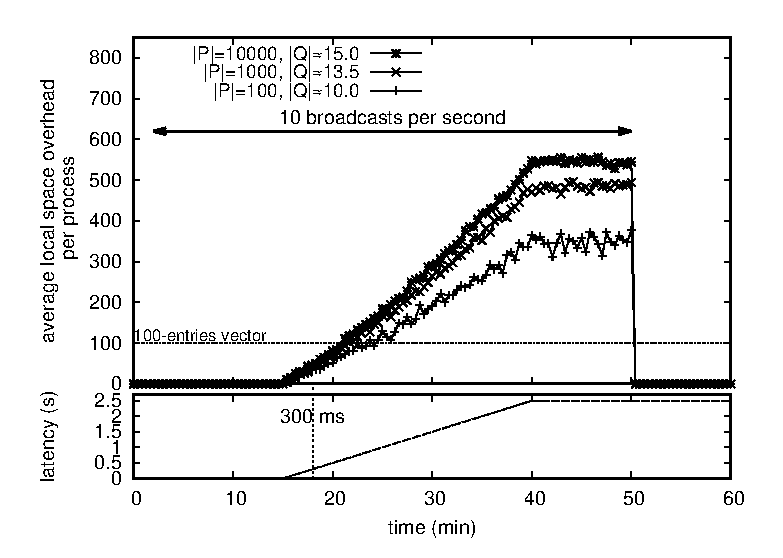
\includegraphics[width=0.8\columnwidth]{./img/overhead.eps}
    \caption{Local space overhead over time.}
  \end{center}
\end{figure}

%%% Local Variables:
%%% mode: latex
%%% TeX-master: "../paper"
%%% End:
